\chapter{Block Ciphers}

\section{The problem of stream ciphers}

The problem is generating a key as long as the plaintext. In block ciphers we encrypt block of bits, typically 64 bits. We do not see the plaintext as a stream of bits, but as collection of blocks. If the plaintext is not divisible by the block size we add padding. Additionally every block is encrypted in isolation or combination and these are called modes of operation.

\section{Introduction to block ciphers}

The main idea is to replace a block of $N$ bits from the plaintext with a block of N bits from the ciphertext. 
\begin{figure}
	\centering
	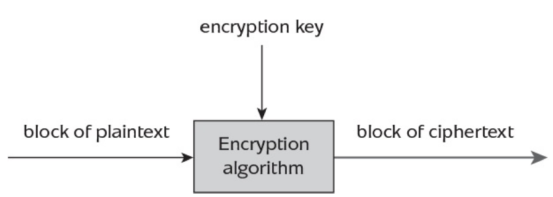
\includegraphics[width=0.4\linewidth]{Images/Chapter3/block_cipher}
	\caption{}
	\label{fig:block_cipher}
\end{figure}

\begin{figure}
	\centering
	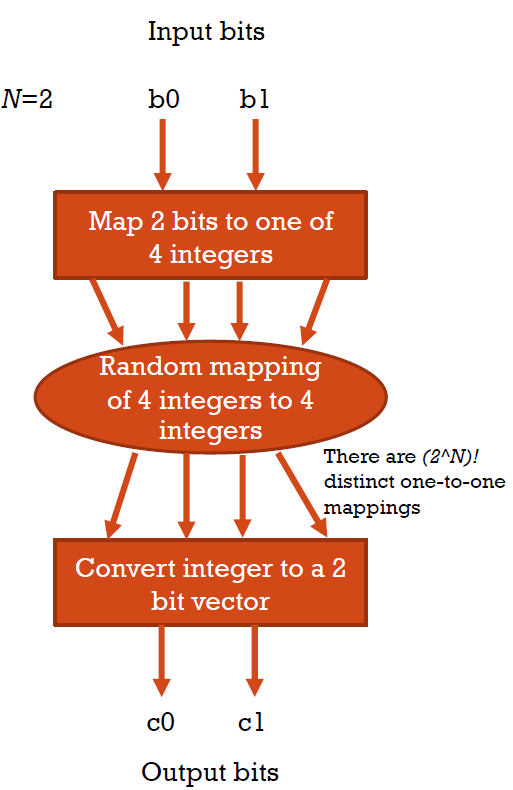
\includegraphics[width=0.3\linewidth]{Images/Chapter3/function_mapping}
	\caption{}
	\label{fig:function_mapping}
\end{figure}

The relationship between the input blocks and the output block is completely random. But it must be invertible for decryption to work. Thus, it has to be one-to-one, i.e. each input block is mapped to a unique output block. Usually, N=64, 128, 256. If the block size is too small, then the number of different plaintext blocks that can ever be encrypted may be too small for an attacker to launch a type of dictionary attack by building up a dictionary of plaintext/ciphertext pairs, if the block size is too large, then the block cipher becomes inefficient to operate, particularly for plaintexts smaller than the block size as they need padding. The encryption key for the ideal block cipher is the table (also called the codebook) that shows the relationship between the input and the output blocks. Think of each possible input block as one of $2^N$ integers and for each such integer we can specify an output $N$-bit block. This means that the encryption key for the ideal block cipher using $N$-bit blocks will be of size $N*(2^N)$. An ideal block cipher is called a random permutation. If $N$ is 64 then the codebook will be of size $N*(2^N)$ which is around $10^{21}$, but this is not practical since we can can not share such keys.

To make this practical a block cipher is a keyed family of pseudorandom permutations. For each key, we have a single permutation that is independent of all the others. Think of each key as corresponding to a different codebook and our strategy is to choose $2^K$ permutations uniformly at random from the set of all $(2^N)!$ permutations. 
We need a 1-to-1 function to map bits to their respective representation \ref{fig:function_mapping}. 
To encrypt we simply divide the plaintext in blocks, and for each block ask the random number generator to return the ciphered block given the plaintext block. During decryption the process is reversed, round keys are used in reverse orderd. 

Block ciphers are slower than stream ciphers but are generally considered more secure than the latter.
Block ciphers have a property called diffusion: 2 blocks differing in a single bit shall generate 2 very different ciphertexts. So even a small transmission error will give rise to errors in around half of the bits in the plaintext. Block ciphers are the basic building block of other cryptographic primitives. Today AES is the reference choice for block ciphers.

\subsection{Examples of block ciphers}

\begin{itemize}
	\item DES: The default block cipher of the 1980s and 1990s, but now considered broken due primarily to its small key size. The two variants based on repeated DES applications commonly known as 3DES are still respected block ciphers, although there are now faster block ciphers available.
	\item AES: A default block cipher based on the encryption algorithm Rijndael which won the AES design competition by NIST to identity the successor of DES
	\item Serpent: A respected block cipher with a block size of 128 bits and key lengths of 128, 192, or 256, which was a finalist with AES in the NIST competition. Considered slower but somehow more secure than AES but not as widely adopted
\end{itemize}


\subsection{Unicity distance}
The unicity distance of a cipher encrypting English plaintexts is the minimum of ciphertext required for a (computationally unlimited) attacker to decrypt a ciphertext uniquely (i.e. to recover the particular key used). For example the ciphertext \textit{FJKFPO} could be \textit{thatis},\textit{season},\textit{ofyour},...

Intuitively, the longer the ciphertext, the fewer possible plaintexts there are that generate the ciphertext. The question is how long does a piece of ciphertext need to be, before it has only one possible decryption? The minimum length is called the unicity distance. And it turns out that the unicity distance depends on the redundancy in the plaintexts.

The unicity distance of a cipher encrypting English plaintexts is the minimum of ciphertext required for a (computationally unlimited) attacker to decrypt a ciphertext uniquely.
Given WNAIW, is it possible to guess a unique plaintext that when a 1-to-1 function is applied to this plaintext we get the ciphertext? No... RIVER and WATER are valid options, but there are many more that are unreasonable ones, because they are not English words (in this case we used a substitution cipher).

We need to take into consideration that the distribution of letters is not uniform. It is redundant, "qu" is more common than "ql", so the redundancy of English has been evaluated to 3.2 bits per character. In English, the substitution cipher has a key that consists of 26 letters since the total number of keys is the number of permutations in which we can arrange 26 letters, is $26!$. The amount of storage (expressed in number of bits) required for all permutations is $log(26!) = 88.28$, so in case of the substitution cipher the unicity distance is $88.28/3.2 = 27.6$. This is because the redundancy of English has been evaluated to be around 3.2 bits per character. In a system with an infinite length random key, it is possible to prove that the unicity distance is infinite.

\textbf{In practice the unicity distance measures the amount of ciphertext required such that there is only one reasonable plaintext.
We want the unicity distance as large as possible.}

Let us generalize a bit by considering a block cipher with a $N$ as the block size and $K$ as the key size. The question becomes then: what is the unicity distance under a known plaintext attack? More formally: given $t$ pairs of plaintexts with corresponding ciphertexts, which is the value of $t$, before it is likely that only one value of the key could have encrypted the plaintext? The answer is the unicity distance, i.e. the number of bits required to express the key space divided by the redundancy in bits per character.

Let's say that Eve intercepts $n$ ciphertexts $c_1, c_2,\ldots$ encrypted from $n$ plaintexts $m_1, m_2,\ldots$ using the same key. Redundancy exists in the messages. There is a value of $n$ equal to the unicity distance such that only one value for the key recreates a possible plaintext (unless Alice and Bob use the One Time Pad).

The observation: the same block with the same key produces always the same output ciphertext independently of its position in a sequence. We will see this is the problem with AES-ECB encryption. The attacker could create a table for each plaintext-ciphertext combination, with one table for each key, but we can defend against this by changing key often, or make sure there are too many keys to try, and thus unicity distance is not reached, and increasing the length of the key to have larger unicity distance and encode with larger blocks, in AES the key size must be at least 128 bits.

Definition of unicity distance under Shannon Theorem assumptions: the minimum amount of ciphertext required to allow a computationally unlimited adversary to recover the unique encryption key. A small unicity distance does not necessarily imply that a block cipher is insecure in practice. Consider a 64-bit block cipher with a unicity distance of two ciphertext blocks: It may still be computationally infeasible for an attacker (of reasonable but bounded computing power) to recover the key, although theoretically there is sufficient information to allow this.

Diffusion means that if we change a single bit of the plaintext, then about half of the bits in the ciphertext should change. Permutations creates diffusion. Ideally, if one bit of the plaintext is changed, then the ciphertext should change completely, in an unpredictable or pseudorandom manner. 
\begin{itemize}
	\item Avalanche criterion: Flipping a fixed set of bits should change each output bit with probability one half
	\item Strict avalanche criterion: For a randomly chosen input, if one flips the $i-th$ bit, then the probability that the $j-th$ output bit will change should be one half, for any $i$ and $j$
\end{itemize}


Confusion means that each bit of the ciphertext should depend on several parts of the key. It refers to making the relationship between the key and the ciphertext as complex and involved as possible. Substitutions creates confusion. This can be achieved by ensuring that the system is nonlinear. Each bit of the ciphertext should depend on the entire key, and in different ways on different bits of the key. Changing one bit of the key should change the ciphertext completely.

Modern block ciphers are typically obtained by mixing substitutions and permutations to obtain both confusion and diffusion.

\section{Anatomy of block ciphers}

A block cipher is a keyed family of pseudorandom permutations. For each key, we have a single permutation that is independent of all the others. The strength of a block ciphers depends on how we design ways to choose $2^K$ permutations uniformly at random from the set of all $(2^N)!$ permutations. For a block cipher to be good, Eve should not be able to recover the key even using multiple plaintext-ciphertext pairs.

Then we create a substitution-permutation network that is simplest way to achieve both diffusion and confusion: the plaintext and the key often have a very similar role in producing the output, hence it is the same mechanism that ensures both diffusion and confusion. It takes a block of the plaintext and the key as inputs, and to produce the ciphertext block applies several alternating "rounds" or "layers" of substitution boxes (S-boxes) and permutation boxes (P-boxes) \ref{fig:DES_Rounds}.

\begin{itemize}
	\item S-Box: It substitutes a small block of bits by another block of bits. Substitution should be one-to-one, to ensure invertibility (hence decryption). An S-box is usually not just a permutation of the bits. Rather, a good S-box will have the property that changing one input bit will change about half of the output bits (with an avalanche effect). It will also have the property that each output bit will depend on every input bit. Could be thought of as a substitution cipher \ref{fig:DES_S_Box}. 
	\item P-Box: Permutation of all bits. Takes the output of S boxes of one round and permutes the bits and feeds them to the next S box. A good P-box has the property that the output bits of any S-box are distributed to as many S-box inputs as possible. Could be thought of as a transposition cipher. \ref{fig:Types_P_Boxes}
\end{itemize}

\begin{figure}
	\centering
	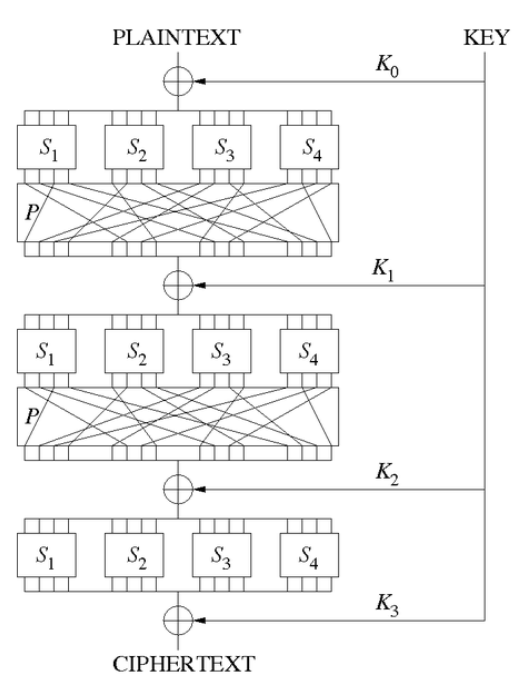
\includegraphics[width=0.7\linewidth]{Images/Chapter3/DES_Rounds}
	\caption{Substitution permutation network}
	\label{fig:DES_Rounds}
\end{figure}


\begin{figure}
	\centering
	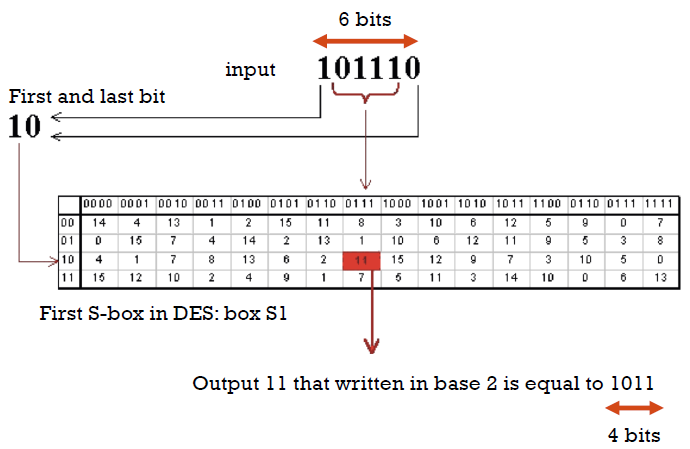
\includegraphics[width=0.7\linewidth]{Images/Chapter3/DES_S_Box}
	\caption{The first S-box in DES}
	\label{fig:DES_S_Box}
\end{figure}


\begin{figure}
	\centering
	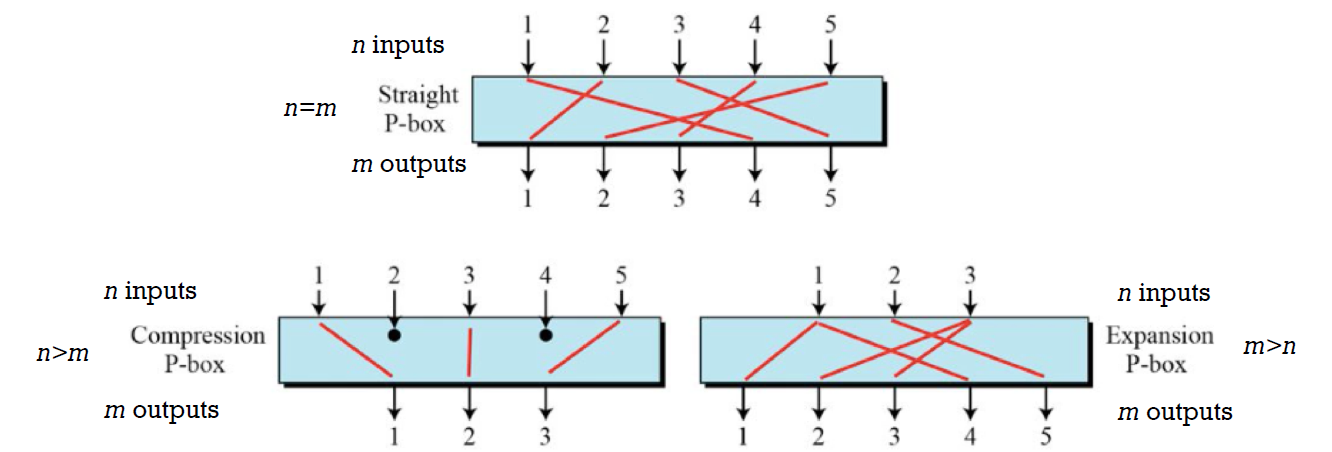
\includegraphics[width=0.7\linewidth]{Images/Chapter3/Types_P_Boxes}
	\caption{P-Box}
	\label{fig:Types_P_Boxes}
\end{figure}

\begin{figure}
	\centering
	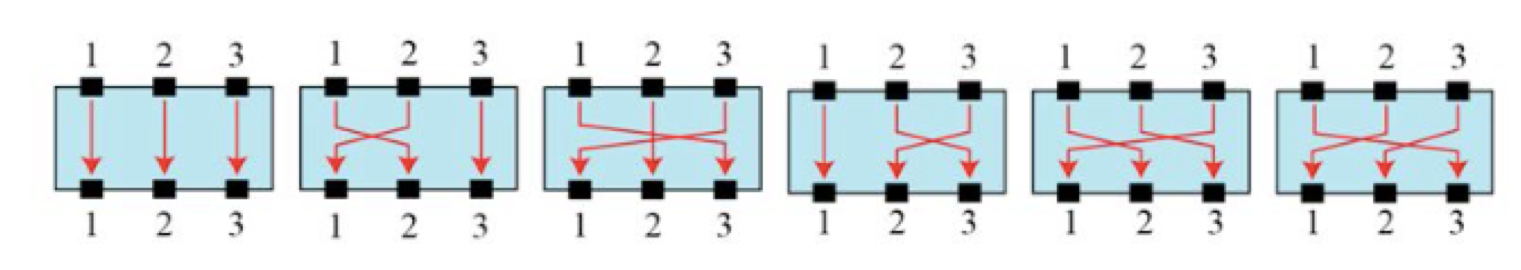
\includegraphics[width=0.7\linewidth]{Images/Chapter3/P_Box_3}
	\caption{Example of P-Box straight of size 3}
	\label{fig:P_Box_3}
\end{figure}

\begin{figure}
	\centering
	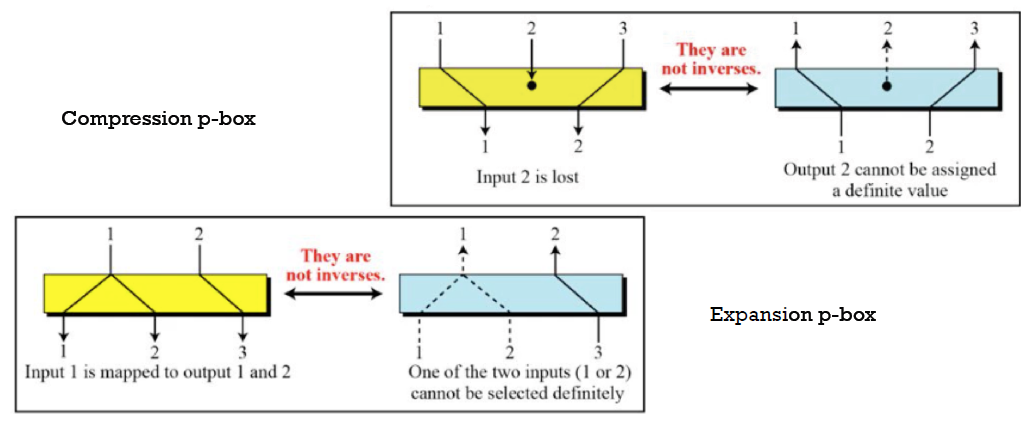
\includegraphics[width=0.7\linewidth]{Images/Chapter3/Expansion_Compression_PBoxes}
	\caption{Types of P-Box}
	\label{fig:Expansion_Compression_PBoxes}
\end{figure}



How we define the numbers in the table \ref{fig:DES_S_Box}? In DES it was a secret, and NSA released some details some time ago, but nobody knows all the detail and how those numbers were chosen. An S-Box may or may not be invertible. When it is, the number $f$ input and output bit should be the same.

A straight P-Box \ref{fig:P_Box_3} is invertible whereas neither a compression nor an expansion P-Box is so \ref{fig:Expansion_Compression_PBoxes}.

\section{DES (Data Encryption Standard)}
Based on the Feistel Structure \ref{fig:DES_FeistelFunction}.
It uses the same basic algorithm for both encryption and decryption. It consists of multiple rounds of processing of the plaintext, with each round consisting of a substitution step followed by a permutation step \ref{fig:DES_Overwiew}. In each round:
\begin{itemize}
	\item the right half of the block, R, goes through unchanged
	\item the left half, L, goes through an operation that depends on R and the encryption key, called round key, derived from the main encryption key
	\item the operation carried out on the left half L is referred to as the Feistel Function F
	\item The permutation step consists of swapping the modified L and R
\end{itemize}

Main advantage of DES is that the same hardware can be used for encryption and decryption. For decryption it is just needed to use the key in the reverse order. In DES the number of rounds is 16 times. The output of each round during decryption is the input to the corresponding round during encryption, except for the left-right switch between the two halves, and this holds true regardless of the choice of the Feistel function $F$. DES uses a 56-bit encryption key.

\begin{figure}
	\centering
	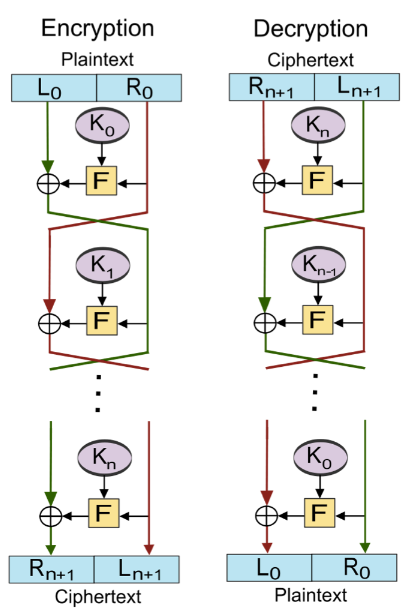
\includegraphics[width=0.7\linewidth]{Images/Chapter3/DES_Overwiew}
	\caption{DES Overview}
	\label{fig:DES_Overwiew}
\end{figure}

\subsection{Feistel function}

The Feistel function \ref{fig:DES_FeistelFunction} is composed of various steps. First the input data is divided in two parts of 32-bits each. Then the right half $RE$ is expanded into a 48-bit block in the Expansion permutation step by attaching a bit at the beginning and a bit at the end of each 4-bit sub-block. The expansion is needed because $RE$ is 32-bits and the key derived by the key scheduling algorithm is 48-bits.
\begin{enumerate}
	\item divide the 32-bit block into eight 4-bit words
	\item attach an additional bit on the left to each 4-bit word that is the last bit of the previous 4-bit word
	\item attach an additional bit to the right of each 4-bit word that is the beginning bit of the next 4-bit word
\end{enumerate}

The second step is called key mixing. And consists of taking the 48 bits of the expanded output produced by the Expansion permutation step and XOR it with the round key, then the output produced is broken into eight 6-bit words. Each 6-bit word goes through a substitution step; its replacement is a 4-bit word. The substitution is carried out with an S-Box. So after all the substitutions, we again end up with a 32-bit word \ref{fig:DES_SubstitutionStep}. Each of the eight S-boxes consists of a 4 × 16 table lookup for an output 4-bit word. The first and the last bit of the 6-bit input word are decoded into one of 4 rows and the middle 4 bits decoded into one of 16 columns for the table lookup. The goal of the substitution carried out by an S-Box is to enhance diffusion \ref{fig:DES_S_Box}.

After, the 32-bits of the previous step then go through a P-box based permutation. What comes out of the P-box \ref{fig:DES_P_Box} is then XOR-ed with the left half of the 64-bit block that we started out with. The output of this XOR operation gives us the right half block for the next round. The table \ref{fig:DES_P_Box} should be read as: the 0th output bit will be the 15th bit of the input, the 1st output bit the 6th bit of the input, and so on for all of the 32 bits of the output that are obtained from the 32 bits of the input.

\begin{figure}
	\centering
	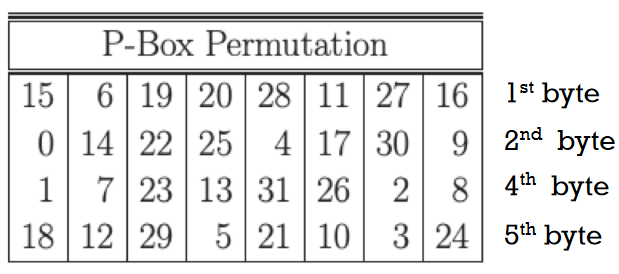
\includegraphics[width=0.3\linewidth]{Images/Chapter3/DES_P_Box}
	\caption{DES P Box}
	\label{fig:DES_P_Box}
\end{figure}

\begin{figure}
	\centering
	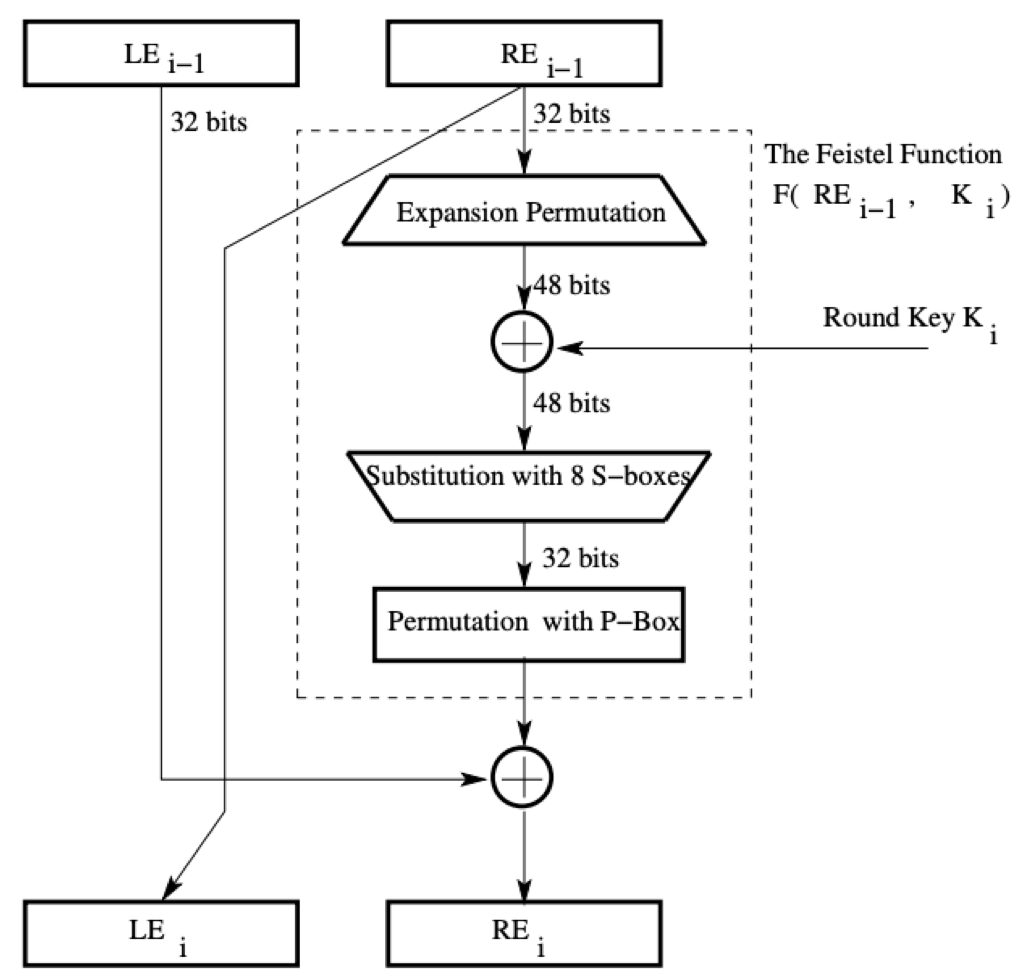
\includegraphics[width=0.7\linewidth]{Images/Chapter3/DES_FeistelFunction}
	\caption{Feistel function}
	\label{fig:DES_FeistelFunction}
\end{figure}

\begin{figure}
	\centering
	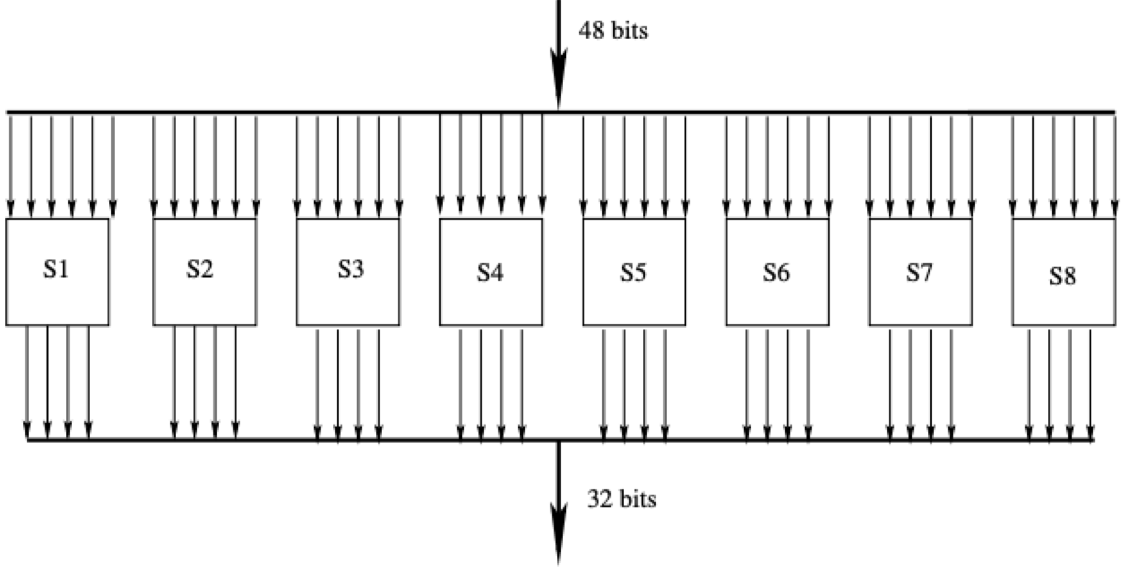
\includegraphics[width=0.7\linewidth]{Images/Chapter3/DES_SubstitutionStep}
	\caption{DES S Box}
	\label{fig:DES_SubstitutionStep}
\end{figure}
\subsection{Differential attacks}

The S-boxes were tuned to enhance the resistance of DES to differential attacks. It is an instance of a chosen plaintext attack. Recall that in a chosen plaintext attack the attacker must be able to obtain ciphertexts for some set of plaintexts of their choosing.
Differential cryptanalysis of block ciphers consists of presenting to the encryption algorithm pairs of plaintext bit patterns with known differences between them and examining the differences between the corresponding ciphertexts. Typically the notion of difference between two plaintexts or ciphertexts is the XOR of the bits performed position-wise.
By feeding into a cipher several pairs of plaintext blocks with known $dX$ (differences in the plaintexts) and observing the corresponding $dY$ (differences in the ciphertexts), it is possible to discover parts of the round keys.


\subsection{DES Key Scheduling}

The 56-bit encryption key is represented by 8 bytes, with the least significant bit of each byte used as a parity bit. The relevant 56 bits are subject to a permutation before any round keys are generated. The table \ref{fig:DES_Key_Scheduling} specifies the 0th bit of the output will be the 56th bit of the input (in a 64 bit representation of the 56-bit encryption key), the 1st bit of the output the 48th bit of the input, and so on, until we have for the 55th bit of the output the 3rd bit of the input.

At the beginning of each round we divide the 56 relevant key bits into two 28 bit halves and circularly shift to the left each half by one or two bits, depending on the round, according to the table \ref{fig:DES_Key_Shift}. The key permutation with the one-bit or two-bit rotation of the two key halves prior to each round aims to ensure that each bit of the original encryption key is used in roughly 14 of the 16 rounds.

For generating the round key, we glue together the two halves and apply a 56 bit to 48 bit contracting permutation (this is referred to as Permutation Choice 2) to the joined bit pattern. The resulting 48 bits constitute the round key \ref{fig:Key_Permutation_2}. The bit addressing now spans the 0 through 55 index values for the 56 bit key. Out of this index range, the permutation shown above retains only 48 bits for the round key. Since there are only six rows and there are 8 positions in each row, the output will consist of 48 bits. The permutation order for the bits is given by reading the entries shown from the upper left corner to the lower right corner.


\begin{figure}
	\centering
	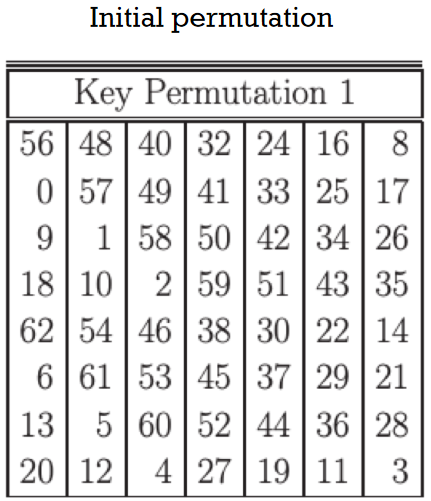
\includegraphics[width=0.3\linewidth]{Images/Chapter3/DES_Key_Scheduling}
	\caption{DES Key Scheduling}
	\label{fig:DES_Key_Scheduling}
\end{figure}

\begin{figure}
	\centering
	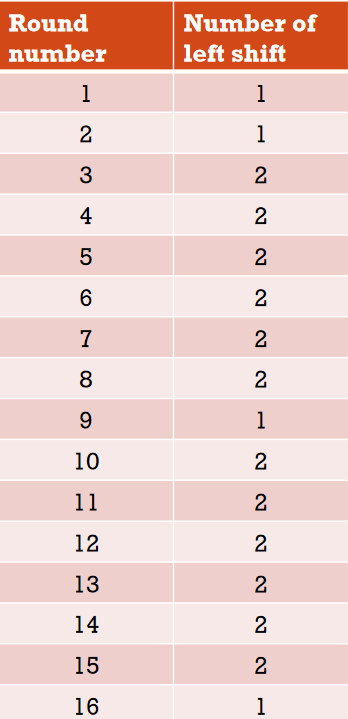
\includegraphics[width=0.2\linewidth]{Images/Chapter3/DES_Key_Shift}
	\caption{DES Key Shift}
	\label{fig:DES_Key_Shift}
\end{figure}

\begin{figure}
	\centering
	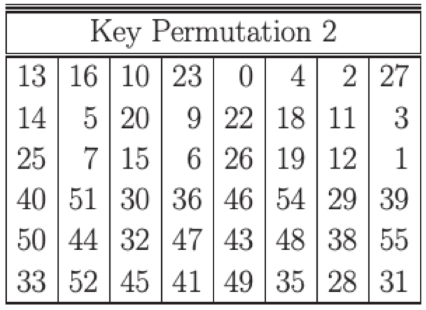
\includegraphics[width=0.3\linewidth]{Images/Chapter3/Key_Permutation_2}
	\caption{Key Permutation 2}
	\label{fig:Key_Permutation_2}
\end{figure}


\subsection{Remarks on DES}
The substitution step is very effective in supporting diffusion: if one changes just one bit of the 64-bit input data block, on the average it propagates out to affect 34 bits of the ciphertext block.
The manner in which the round keys are generated
from the encryption key is also very effective in supporting confusion: if one changes just one bit of the encryption key, on the average that affects 35 bits of the ciphertext.

The 56-bit encryption key means a key space of size $2^{56} \approx 7.2 * 10^{16}$. In a brute-force attack, a machine able to process 1,000 keys per microsecond would need roughly 13 months to break the code. But the EFF in 1999 created a computer that was able to enumerate the $2^{56}$ keyspace and crack DES in just 10 hours. So DES was deprecated, but not immediately, before they issued a call for defining a new standard, but it took several years because cryptographers needed to scrutinize the algorithm, and for the time beign NIST issued a new directive that year that required organizations to use Triple DES, i.e. 3 consecutive applications of DES \ref{fig:3DES}, and it is still used today!

\begin{figure}
	\centering
	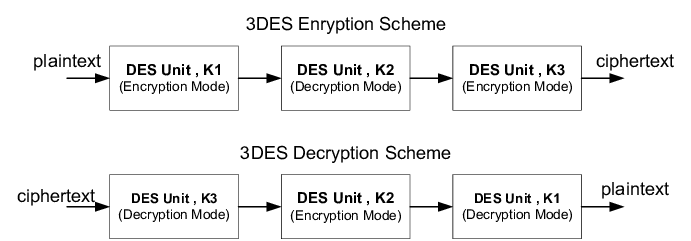
\includegraphics[width=0.7\linewidth]{Images/Chapter3/3DES}
	\caption{3DES}
	\label{fig:3DES}
\end{figure}

To understand why triple DES was chosen and not just Double DES we need to take into consideration the Meet-In-The-Middle attack. 

\subsection{DoubleDES and the Meet-In-The-Middle attack}

A naive approach to increase the strength of a block cipher with short keys is to use two keys $k_1$ and $k_2$ instead of one and encrypt the block twice with them. The hope is that the scheme will provide the same security of using a key of length $k_1+k_2$. This is not the case because of the meet-in-the-middle attack where insted of performing $2^{k_1+k_2}$ guesses, the attacker only needs to perform $2^{k_1 + 1} = 2^{k_1} + 2^{k_2}$ guesses, let $C=ENC_{k_2}(ENC_{k_1}(P))$ and $P=DEC_{k_2}(DEC_{k_1}(C))$:
\[C=ENC_{k_2}(ENC_{k_1}(P))\]
\[DEC_{k_2}(C)=DEC_{k_2}(ENC_{k_2}(ENC_{k_1}(P)))\]
\[DEC_{k_2}(C)=ENC_{k_1}(P)\]

Now consider the two sides of the equality: $DEC_{k_2}(C)=ENC_{k_1}(P)$, the attacker can compute $DEC_{k_2}(C)$ for all possible values of $k_2$, then compute $ENC_{k_1}(P)$ for all possible values of $k_1$ for a total of $2^{k_1} + 2^{k_2}$ or $2^{k_1 + 1}$ if $k_1$ and $k_2$ are the same size operations. If the result from any of the $ENC_{k_1}(P)$ operations matches a result from the $DEC_{k_2}(C)$ operations, the pair of $k_1$ and $k_2$ is possibly the correct key, called a candidate key. The complexity difference compared to the bruteforce method is quite significant: $2^{k_1 + k_2} = 2^{k_1} * 2^{k_2}$ versus $2^{k_1 + 1} = 2^{k_1} + 2^{k_2}$.

\section{Triple DES}

Triple DES uses a key bundle comprising 3 DES keys ($k_1$, $k_2$, $k_3$), each one of 56 bits length. Encryption works as follows: 
$E_{k_3}(D_{k_2}(E_{k_1}(P)))$. Decryption is the inverse: $D_{k_1}(E_{k_2}(D_{k_3}(C)))$. Each triple encryption works on blocks of 64 bits of data.
In each case the middle operation is the reverse of the first and last. This improves the strength of the algorithm when using keying option 2 and provides backward compatibility with DES with keying option 3. 

\subsection{Choosing Keys for Triple DES}

Choosing keys; Care should be put in selecting the keys in key bundle
\begin{itemize}
	\item All three keys are independent. Strongest option, still vulnerable to meet-in-the-middle but requires $2^{2*56} = 2^{112} \approx 5.19 * 10^{29}$ operations
	\item $k_1$ and $k_2$ are independent but $k_3=k_1$. Similar to double DES and vulnerable to the same attack with equal complexity, deprecated
	\item All three keys are equal. For backward compatibility with DES, since two operations cancel out, forbidden because equal to DES
\end{itemize}

Additionally, some specific values for keys are forbidden. With these restrictions, Triple DES has been reapproved with keying options 1 and 2 only although it is current best practice to use only option 1 as keys should be generated by using random generators.


\section{AES (Advanced Encryption Standard)}

Notified by NIST as a standard in 2001, it has a block length 128bits. The key scheduling (how you derive the keys in each round) changes based on the key length: 10 rounds for 128-bit keys, 12 rounds for 192-bit keys and 14 rounds for 256-bits keys. Except for the last round, all other rounds are identical. 


Unlike DES, AES is an example of key-alternating block ciphers: each round first applies a diffusion-achieving transformation operation to the entire incoming block, which is then followed by the application of the round key to the entire block.
DES is based on the Feistel structure in which, for each round, one-half of the block passes through unchanged and the other half goes through a transformation that depends on the S-boxes and the round key.
Key alternating ciphers lend themselves well to theoretical analysis of the security of the ciphers.

\subsection{AES Round: Encryption}

Each round includes
\begin{enumerate}
	\item one single-key based substitution step
	\item a row-wise permutation step
	\item a column-wise mixing step
	\item the addition of the round key
\end{enumerate}

The order of these steps is different for encryption and decryption. Each round takes an input state array and returns an output state array. The output state array produced by the last round is rearranged into a 128-bit output block.
Unlike DES, decryption differs substantially from encryption although similar transformations are used. One bit change of the input introduces dramatic changes in the output ciphertext.

DES is based on the Feistel (substitution-permutation) network. DES involves substitutions and permutations. Permutations are based on the Feistel notion of dividing the input block into two halves, processing each half separately, and then swapping the two halves.

AES uses a substitution-permutation network in a more general sense. Each round in AES involves key-level substitutions followed by word-level permutations. Like DES, AES is an iterated block cipher in which plaintext is subject to multiple rounds with each round applying the same overall transformation function to the incoming block.

\subsection{Structure of AES}

The 128 bits key is arranged in the form of an array of $4 * 4$ keys. The four column words of the key array are expanded into a schedule of 44 words.  Each round consumes four words from the key schedule (recall that AES has 10 rounds with a key length of 128 bits). The first 4 words are used for adding to the input state array before any round can begin. The remaining 40 words are used for the 10 rounds.
Recall that key expansion generates 44 keys. The first 4 are mixed with the input blocks (AddRoundKey).
\begin{itemize}
	\item Encryption: the input state array is XOR-ed with the first four words of the key schedule.
	\item Decryption: same as above except that the ciphertext state array is XOR-ed with the last four words of the key schedule
\end{itemize}
The remaining 40 are used in each one of the 10 rounds 4 at a time. We are using tables in AES, and in decryption the inverse of those tables.

\subsection{Structure of a round}
There are some encryption steps: Substitute bytes, Shift rows, Mix columns, Add round key, and decryption steps: Inverse shift rows, Inverse substitute bytes, Add round key, Inverse mix columns. The final round for encryption does not involve the Mix columns step. The final round for decryption does not involve the Inverse mix columns step.
In the case of AES-128, the 128 bits are organized as a $4$x$4$ array of cells, where each cell is made up of eight bit.

\subsection{Round Steps}

\subsubsection{Round Step 1}

\texttt{SubBytes} for byte-by-byte substitution during encryption. \texttt{InvSubBytes} for the corresponding substitution during decryption. It consists of using a $16$x$16$ lookup table to find a replacement byte for a given byte in the input state array. The entries in the lookup table are created by using the notions of multiplicative inverses in $GF(2^8)$ and bit scrambling to eliminate the bit-level correlations inside each byte \ref{fig:LookupTable}.

\begin{figure}
	\centering
	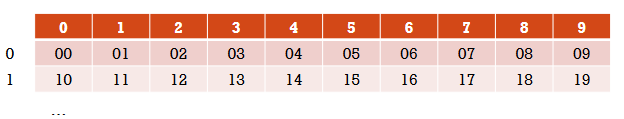
\includegraphics[width=0.7\linewidth]{Images/Chapter3/LookupTable}
	\caption{Round Step 1}
	\label{fig:LookupTable}
\end{figure}

The table is filled in a precise way, in DES it was a secret. Replace the value in each cell by its multiplicative inverse in $GF(2^8)$ based on the irreducible polynomial $x^8 + x^4 + x^3 + x + 1$. 00 has no multiplicative inverse so it is just replaced by itself. With the mapping considered above, the 00 input byte is mapped to c i.e. 0x63 and, at the same time, all other bytes are mapped one-to-one. Why 0x63? Because it works in practice. The table created must be thought of as an S-Box. The main requirement is that the table must be invertible for decryption.

\subsubsection{Round Step 2}

Remember that the state of AES is a matrix. \texttt{ShiftRows} for shifting the rows of the state array during encryption. \texttt{InvShiftRows} for the corresponding transformation during decryption. 

ShiftRows transformation consists of \ref{fig:Round_Step2}: 
\begin{enumerate}
	\item not shifting the first row of the state array at all
	\item circularly shifting the second row by one byte to the left
	\item circularly shifting the third row by two bytes to the left
	\item circularly shifting the last row by three bytes to the left
\end{enumerate}

We are scrambling! Permuting data. For decryption, the corresponding step shifts the rows in exactly the opposite direction.

\begin{figure}
	\centering
	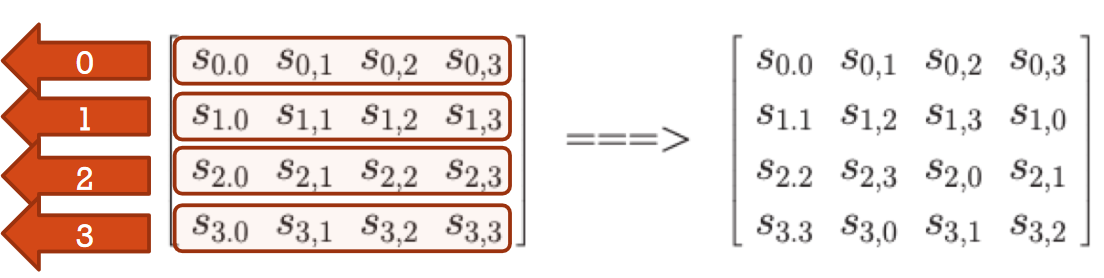
\includegraphics[width=0.7\linewidth]{Images/Chapter3/Round_Step2}
	\caption{Round step 2}
	\label{fig:Round_Step2}
\end{figure}


\subsubsection{Round Step 3}

\texttt{MixColumns} for mixing up of the bytes in each column separately during encryption. \texttt{InvMixColumns} for the corresponding transformation during decryption. This is the 3rd step in encryption and 4th in decryption! This step replaces each byte of a column by a function of all the bytes in the same column. The combination of the shift-rows and the mix-column steps causes each bit of the ciphertext to depend on every bit of the plaintext after 10 rounds of processing. In DES, one bit of plaintext affected roughly 31 bits of ciphertext. In AES, the goal is that each bit of the plaintext will affect every bit position of the ciphertext block of 128 bits. The operation in \ref{fig:Round_Step3} should be read as: each byte in a column is replaced by two times that byte, plus three times the next byte, plus the byte that comes next, plus the byte that follows. The operation must be carried out in $GF(2^8)$, For instance, 'two times' means multiplication by bit pattern $000000010$ ($x$) and 'three times' by bit pattern $00000011$ ($x + 1$). The words 'next' and 'follow' refer to bytes in the same column, and their meaning is circular, in the sense that the byte that is next to the one in the last row is the one in the first row. This fixed matrix is invertible over $GF(2^8)$ so that the entire transformation is invertible.


\begin{figure}
	\centering
	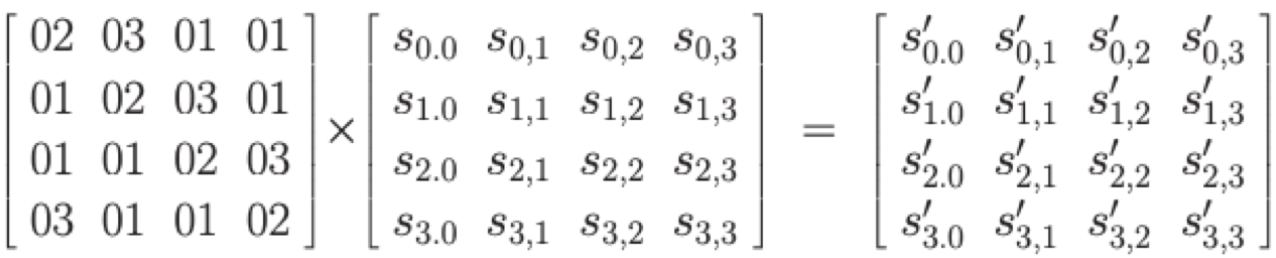
\includegraphics[width=0.7\linewidth]{Images/Chapter3/Round_Step3}
	\caption{Round step 3}
	\label{fig:Round_Step3}
\end{figure}

\subsubsection{Round Step 4}

\texttt{AddRoundKeys} for adding the round key to the output of the previous step during encryption. This is the 4th step in encryption and 3rd in decryption! \texttt{AddRoundKey} or \texttt{InvAddRoundKey} for inverse add round key transformation during decryption. 


\subsection{Key Expansion}

Each round has its own round key that is derived from the original 128-bit encryption key as described in the following. One of the four steps of each round, for both encryption and decryption, involves the XOR-ing of the round key with the state array. The AES Key Expansion algorithm is used to derive the 128-bit round key for each round from the original 128-bit encryption key. The logic of the key expansion algorithm is designed to ensure that if one changes one bit of the encryption key, it should affect the round keys for several rounds.

In the same manner as the 128-bit input block is arranged in the form of a state array, the algorithm first arranges the 16 bytes of the encryption key in the form of a 4 x 4 array of bytes \ref{fig:Key_Expansion_Algorithm1}. 

The first four bytes of the encryption key constitute the word $w_0$. The next four bytes the word $w_1$. The next four bytes the word $w_2$. The last four bytes the word $w_3$. The algorithm subsequently expands the words $w_0,w_1,w_2,w_3$ into a 44-word key schedule $w_0,w_1,\ldots,w_{42},w_{43}$ \ref{fig:Key_Expansion_Algorithm2}.

\begin{figure}
	\centering
	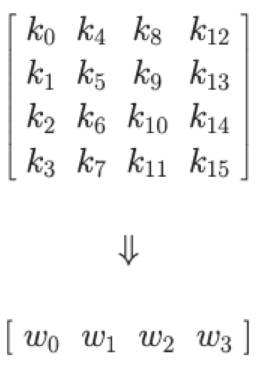
\includegraphics[width=0.4\linewidth]{Images/Chapter3/Key_Expansion_Algorithm1}
	\caption{Key Expansion Algorithm}
	\label{fig:Key_Expansion_Algorithm1}
\end{figure}

\begin{figure}
	\centering
	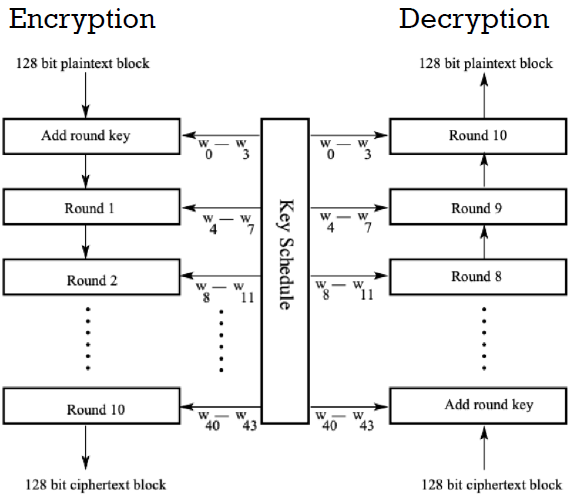
\includegraphics[width=0.7\linewidth]{Images/Chapter3/Key_Expansion_Algorithm2}
	\caption{Key Expansion Algorithm}
	\label{fig:Key_Expansion_Algorithm2}
\end{figure}


But how does the Key Expansion Algorithm expands four words $w_1,w_2,w_3,w_4$ into 44 words $w_0,w_1,\ldots,w_{42},w_{43}$? On a high level the key expansion algorithm works like this: the key expansion takes place on a 4-word to 4-word basis, in the sense that each grouping of 4 words decides what the next grouping of 4 words will be. Let's say we have four words of the round key for the $i$-th round: $w(i),w(i+1),w(i+1),w(i+3)$ we want to generate $w(i+4),w(i+5),w(i+6),w(i+7)$.
Function $g$ takes the four words and returns a single word that is then XOR-ed with each word and we get the words of the next round \ref{fig:Key_Expansion_Algorithm3}.
Except for the first word in a new 4-word grouping, each word is obtained by XOR-ing the previous word and the corresponding word in the previous 4-word grouping.
Mathematically, the transformation is expressed as follows:

\begin{itemize}
	\item $w_{i+4} = g(w_{i+3}) \oplus w_i$
	\item $w_{i+5} = w_{i+4} \oplus w_{i+1}$
	\item $w_{i+6} = w_{i+5} \oplus w_{i+2}$
	\item $w_{i+7} = w_{i+6} \oplus w_{i+3}$
\end{itemize}

\begin{figure}
	\centering
	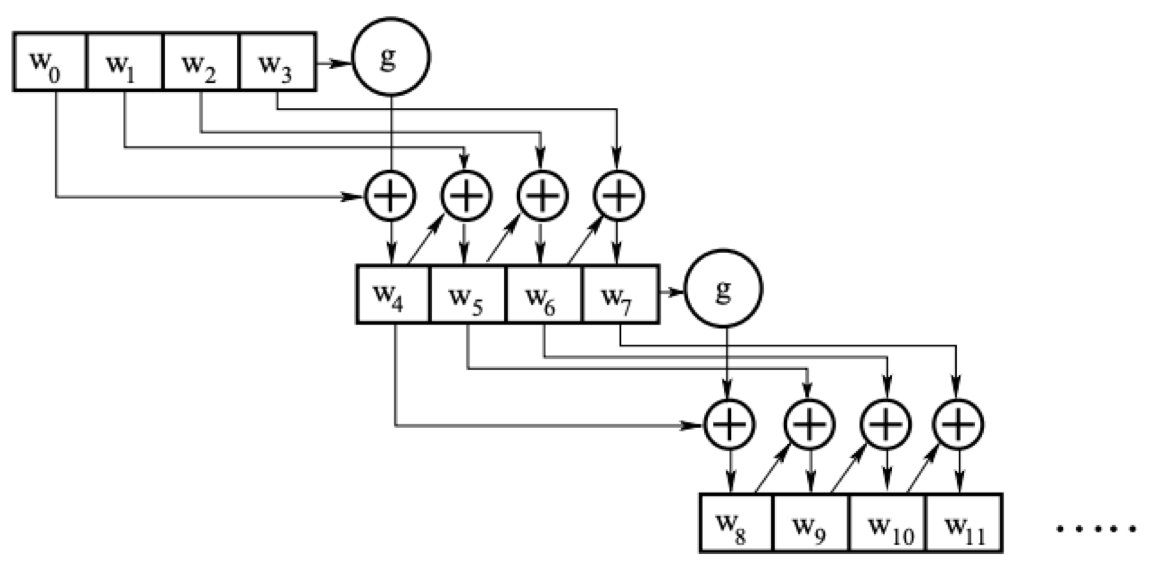
\includegraphics[width=0.7\linewidth]{Images/Chapter3/Key_Expansion_Algorithm3}
	\caption{Key Expansion Algorithm}
	\label{fig:Key_Expansion_Algorithm3}
\end{figure}



The function $g$ consists of the following three steps:
\begin{itemize}
	\item[1.] Perform a one-byte left circular rotation on the argument 4-byte word
	\item[2.] Perform a byte substitution for each byte of the word returned by the previous step by using the same 16 x 16 lookup table as used in the SubBytes step of the encryption rounds
	\item[3.] XOR the bytes obtained from the previous step with a round constant. The round constant is a word whose three rightmost bytes are always zero and XOR-ing with the round constant amounts to XOR-ing with just its leftmost byte
\end{itemize}

The key expansion algorithm ensures that AES has no weak keys.

\subsection{Security of AES}
Cryptographers are constantly probing AES for weaknesses. This is essential, because if it was not being thoroughly tested by academics, then criminals or nation states could eventually find a way to crack it without the rest of the world knowing. 


In 2009, a series of related-key attacks were discovered. These involve observing how a cipher operates under different keys. These attacks are only possible against protocols that are not implemented properly.

In 2009, there was a known-key distinguishing attack against an eight round version of AES-128. This attack uses a key that is already known in order to figure out the inherent structure of the cipher. As this attack was only against an eight round version, there is not much to worry about for everyday users of AES-128.

So far, researchers have only uncovered theoretical breaks and side channel attacks. This means that AES is essentially unbreakable at the moment.

\section{Modes of operation for block ciphers}

\subsection{Electronic codebook (ECB)}

\begin{figure}
	\centering
	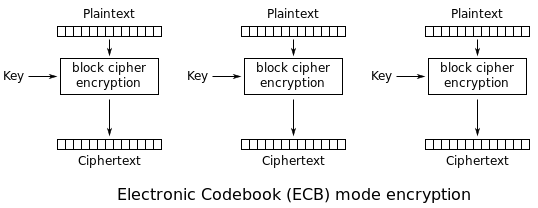
\includegraphics[width=0.7\linewidth]{Images/Chapter3/ECB_Encryption}
	\caption{ECB Encryption}
	\label{fig:ECB_Encryption}
\end{figure}

\begin{figure}
	\centering
	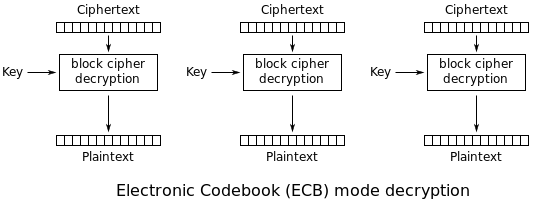
\includegraphics[width=0.7\linewidth]{Images/Chapter3/ECB_Decryption}
	\caption{ECB Decryption}
	\label{fig:ECB_Decryption}
\end{figure}

When a block cipher is used in ECB mode, each block of plaintext is coded independently. This makes it not very secure for long segments of plaintext, especially plaintext containing repetitive information. Primarily used for secure transmission of short pieces of information, e.g., encryption keys. When each block of a plaintext file is encrypted independently of the other blocks, the structure of the information in the ciphertext file can hold important clues to what is in the plaintext file. Given a key, a block cipher always encrypts the same contents the same way. At first, this does not seem to be a problem because the output is still encrypted but it can reveal information, for example a picture \ref{fig:ECB_Fail} even if encrypted with ECB the repeating patters still show, in the picture we can clearly distinguish the text and the background. ECB mode block encryption can leave too many clues in the ciphertext for an attacker. As a consequence, the ECB mode is good only for short messages or messages without too much repetitive structure Another shortcoming of ECB is that the length of the plaintext message must be integral multiple of the block size, if this condition is not met the plaintext must be padded \ref{fig:ECB_Encryption} \ref{fig:ECB_Decryption} .

\begin{figure}
	\centering
	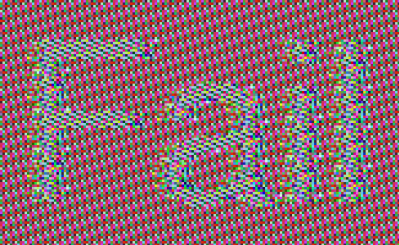
\includegraphics[width=0.7\linewidth]{Images/Chapter3/ECB_Fail}
	\caption{ECB Fail}
	\label{fig:ECB_Fail}
\end{figure}


\subsection{Cipher block chaining (CBC)}

To overcome the security problems of the ECB mode, the input to the encryption algorithm consists of the XOR of the plaintext block and the ciphertext produced from the previous plaintext block. This makes it difficult to identify patterns in the ciphertext that may correspond to the known structure of the plaintext. The chaining scheme shown in the figure needs an Initialization Vector (IV) for the first invocation of the encryption algorithm. The IV is sent separately as a short message using the ECB mode. With CBC, the ciphertext block for any given plaintext block becomes a function of all the previous ciphertext blocks \ref{fig:CBC_Encryption} \ref{fig:CBC_Decryption}.

\begin{figure}
	\centering
	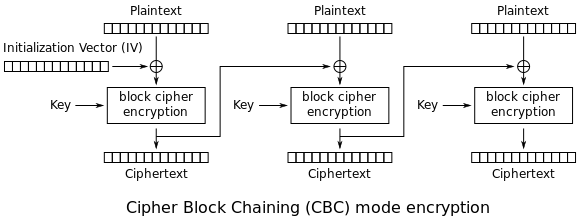
\includegraphics[width=0.7\linewidth]{Images/Chapter3/CBC_Encryption}
	\caption{CBC Encryption}
	\label{fig:CBC_Encryption}
\end{figure}

\begin{figure}
	\centering
	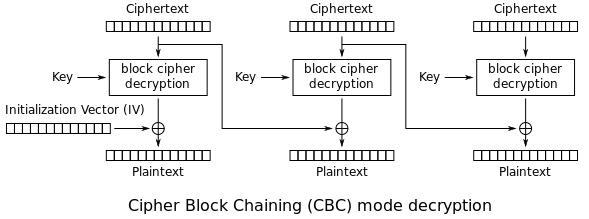
\includegraphics[width=0.7\linewidth]{Images/Chapter3/CBC_Decryption}
	\caption{CBC Decryption}
	\label{fig:CBC_Decryption}
\end{figure}

\subsection{Counter (CTR)}

Counter mode turns a block cipher into a stream cipher. It generates the next keystream block by encrypting successive values of a "counter". The counter can be any function which produces a sequence which is guaranteed not to repeat for a long time, although an actual increment-by-one counter is the simplest and most popular. Notice that only the encryption
algorithm is used in both encryption and decryption. This can be an important implementation-level detail for those block ciphers for which the encryption and the decryption algorithms are significantly different such as AES \ref{fig:CTR_Encryption} \ref{fig:CTR_Decryption}.

\begin{figure}
	\centering
	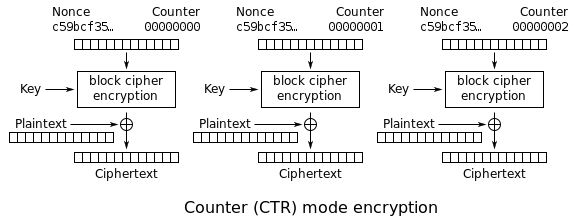
\includegraphics[width=0.7\linewidth]{Images/Chapter3/CTR_Encryption}
	\caption{CTR Encryption}
	\label{fig:CTR_Encryption}
\end{figure}

\begin{figure}
	\centering
	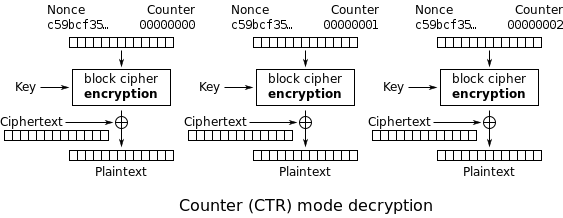
\includegraphics[width=0.7\linewidth]{Images/Chapter3/CTR_Decryption}
	\caption{CTR Decryption}
	\label{fig:CTR_Decryption}
\end{figure}

\subsection{Cipher feedback (CFB)}
\label{sec:CipherFeedback}
The cipher feedback (CFB) mode, in its simplest form uses the entire output of the block cipher. In this variation, it is very similar to CBC, makes a block cipher into a self-synchronizing stream cipher \ref{fig:CFB_Encryption} \ref{fig:CFB_Decryption}.  Notice that only the encryption algorithm is used in both encryption and decryption.
\begin{figure}
	\centering
	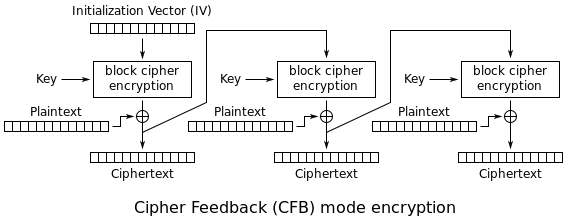
\includegraphics[width=0.7\linewidth]{Images/Chapter3/CFB_Encryption}
	\caption{CFB Encryption}
	\label{fig:CFB_Encryption}
\end{figure}

\begin{figure}
	\centering
	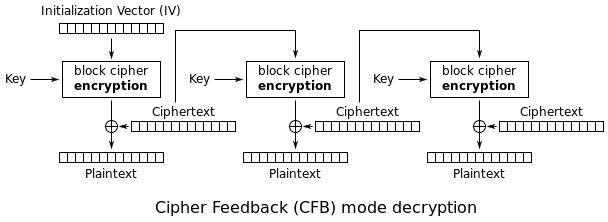
\includegraphics[width=0.7\linewidth]{Images/Chapter3/CFB_Decryption}
	\caption{CFB Decryption}
	\label{fig:CFB_Decryption}
\end{figure}

\subsection{Output feedback (OFB)}

The output feedback (OFB) mode makes a block cipher into a synchronous stream cipher. It generates keystream blocks, which are then XOR-ed with the plaintext blocks to get the ciphertext. Just as with other stream ciphers, flipping a bit in the ciphertext produces a flipped bit in the plaintext at the same location. This property allows many error-correcting codes to function normally even when applied before encryption \ref{fig:OFB_Encryption} \ref{fig:OFB_Decryption}.  Notice that only the encryption
algorithm is used in both encryption and decryption.

\begin{figure}
	\centering
	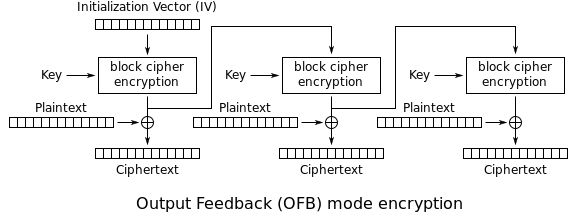
\includegraphics[width=0.7\linewidth]{Images/Chapter3/OFB_Encryption}
	\caption{}
	\label{fig:OFB_Encryption}
\end{figure}

\begin{figure}
	\centering
	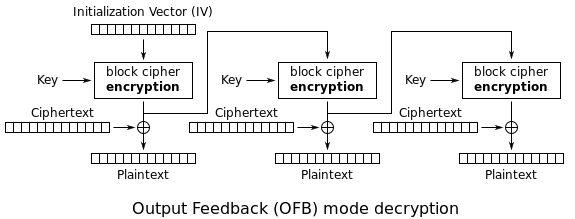
\includegraphics[width=0.7\linewidth]{Images/Chapter3/OFB_Decryption}
	\caption{}
	\label{fig:OFB_Decryption}
\end{figure}

\subsection{Galois/counter mode (GCM)}

Galois/counter mode (GCM) combines the well-known counter mode of encryption with the new Galois mode of authentication. The key feature is the ease of parallel computation of the Galois field multiplication used for authentication. This feature permits higher throughput than encryption algorithms and GCM is defined for block ciphers with a block size of 128 bits. Widely used today in many protocols such as TLS.

Like in CTR, blocks are numbered sequentially. The block number is combined with an IV and encrypted with a block cipher (usually AES). The result of this encryption is XOR-ed with the plaintext to produce the ciphertext \ref{fig:GCM_mode}. Like all counter modes, this is essentially a stream cipher, and so it is essential that a different IV is used for each stream that is encrypted. The ciphertext blocks are considered coefficients of a polynomial which are then manipulated in the corresponding Galois field. The result is then encrypted, producing an authentication tag that can be used to verify the integrity of the data.

\begin{figure}
	\centering
	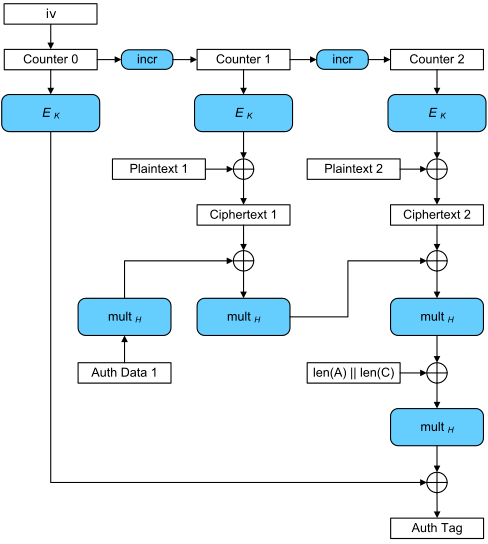
\includegraphics[width=0.7\linewidth]{Images/Chapter3/GCM_mode}
	\caption{GCM Mode}
	\label{fig:GCM_mode}
\end{figure}


\section{DES vs AES}

The basic difference between DES and AES is that the block in DES is divided into two halves before further processing whereas in AES entire block is processed to obtain ciphertext. The DES algorithm works on the Feistel Cipher principle and the AES algorithm works on substitution and permutation principle. The key size of DES is 56 bit which is comparatively smaller than AES which has 128,192, or 256-bit secret key. The rounds in DES include Expansion Permutation, XOR, S-Box, P-Box, XOR and Swap whereas rounds in AES include Subbytes, Shiftrows, Mix columns, Addroundkeys. DES is less secure than AES because of the small key size and the relatively small block size. AES is comparatively faster than DES.
